\documentclass[12pt,a4paper,openany]{report}
\usepackage[utf8]{inputenc}
\usepackage{ucs}
\usepackage[T1]{fontenc}
\usepackage{graphicx}
\usepackage[francais]{babel} 
\usepackage{array} 
\usepackage{color,colortbl}
\usepackage{hyperref}%pour faire des ancres Table des matières -> partie A | partie B | etc

%permet les subsubsubsection :)
\setcounter{secnumdepth}{4}
\setcounter{tocdepth}{3}
\makeatletter
\newcounter {subsubsubsection}[subsubsection]
\renewcommand\thesubsubsubsection{\thesubsubsection .\@alph\c@subsubsubsection}
\newcommand\subsubsubsection{\@startsection{subsubsubsection}{4}{\z@}%
                                     {-3.25ex\@plus -1ex \@minus -.2ex}%
                                     {1.5ex \@plus .2ex}%
                                     {\normalfont\normalsize\bfseries}}
\newcommand*\l@subsubsubsection{\@dottedtocline{3}{10.0em}{4.1em}}
\newcommand*{\subsubsubsectionmark}[1]{}
\makeatother

\title{Etat de l'art}
\author{Projet DUT INFO}
\date{17 Septembre 2013}

\begin{document}

\maketitle

\hypertarget{tableofcontents}{} %affecte des ancres aux differentes partie
\tableofcontents

\part{Introduction}

\chapter{Fonctionnement de l'affichage sur ordinateur}
\section{La carte graphique}
\subsection{Définition}
Une carte graphique, ou carte vidéo, est un périphérique permettant à un ordinateur de communiquer 
avec un écran.\\
\subsection{Composants}
\textbf{GPU} (Graphical Processing Unit) : Processeur graphique, constituant le cœur de la carte graphique, et qui possède des instructions évoluées de traitement d’image. Un GPU est une unité de calcul massivement parallèle.\\\\
\textbf{Mémoire vidéo} (Frame Buffer) : Conserve les images traitées par le GPU avant l’affichage.
\subsection{Fonctionnement en mode texte}
Les premières cartes graphiques datent du début des années 1980, à une époque à laquelle les ordinateurs n'affichaient que du texte à l'écran.\\
Ces cartes ne permettaient d'afficher à l'écran qu'une grille de caractères 
(25 lignes de 80 caractères) prédéfinis qui mesuraient 9x14 pixels chacun. Il était ainsi impossible de modifier directement la valeur d'un pixel.\\
Ce mode de fonctionnement ainsi que la table des caractères utilisables est 
définie par la norme MDA, "Monochrome Display Adapter"\footnote{http://www.seasip.info/VintagePC/mda.html}
du nom de la carte graphique d'IBM qui inaugura cette technologie.\\
Il est à noter que c'est le CPU\footnote{Central Processing Unit : Unité de calcul centrale / Processeur de la machine} qui donnait ses instructions à la carte graphique, celle-ci ne faisant que transmettre les caractères à l'écran.\\
Cette norme est encore utilisée de nos jours, elle permet notamment au BIOS d'afficher des informations au démarrage d'un ordinateur.

\subsection{Fonctionnement en mode graphique}

En 1981 apparait la première carte graphique permettant d'adresser chaque pixel de l'écran indépendamment.
Fabriquée par IBM, cette carte dite CGA, "Color Graphic Adapter" permettait d'utiliser une résolution de 320 par 200 pixels en mode 4 couleurs ou une résolution de 640 par 200 pixels en mode monochrome.\\
Cette carte est une avancée majeure puisqu'elle permet désormais d'afficher n'importe qu'elle forme à l'écran, et plus uniquement des caractères. C'est le début de l'informatique graphique.

\subsection{L'accélération matérielle 2D}

A l'époque, le rôle de la carte graphique se limitait à servir d'intermédiaire entre le CPU et l'écran, c'était le rôle du CPU de définir l'ensemble des pixels à afficher. Par exemple si une application souhaitait tracer une ligne entre deux points A et B, le CPU devait alors calculer la position de chaque pixel composant la ligne avant de demander à la carte graphique d'afficher ceux-ci.\\
Aussi durant les années 1980, avec l'arrivée des interfaces graphiques, les cartes graphiques devinrent de plus en plus performantes dans le but de délester le CPU : elles étaient désormais capables de tracer elles-mêmes des primitives géométriques simples telles que des lignes, des triangles, des rectangles, des cercles, voire de colorier celles-ci d'après les consignes données par le CPU.\\

\subsection{Historique des GPU}
\begin{center}
\begin{tabular}{|c|c|m{0.2\linewidth}|m{0.3\linewidth} |c|}
\hline
Année & Génération & Carte & Application & Bus \\
\hline
1996 & 1 & 3dfx Voodoo & texture mapping et z-buffer & bus PCI\\
\hline
1998 & 2 & GeForce/ Radeon 7500 & Transform\&lighting, multi-texting & bus AGP \\
\cline{1-4}
2001 & 3 & GeForce3/ Radeon 8500 & Programmation sur les sommets (vertex shader)	& \\
\cline{1-4}
2002 & 4 & Radeon 9700/GeForce FX & Programmation sur les pixels (fragment shader)	& \\
\hline
2008 & 5 & GeForce9/ Radeon HD & Compatibilité OpenGL et DirectX,  geometry shader & bus PCIe \\
\hline
\end{tabular}
\end{center}

Les bus PCI(Peripheral Component Interconnect), AGP(Advanced Graphics Port) et  PCIexpress sont des bus local.
Bus local : système de communication entre des cartes d’extension et la carte mère.
Le bus PCIe est une version plus petite et plus performante que le PCI et AGP.


\part{Pipeline graphique}
\section{Définition}
Un pipeline (tuyau) graphique est une succession de tâches réalisées par la carte graphique nécessaires à la création de données géométriques afin de produire une scène 3D.
\\\\
En entrée, il récupère des coordonnées de points, et en sortie, il renvoi des Texels (TExtured piXEL).
\\
\textbf{Le texel} est un ou plusieurs pixels, sur les quelles, une texture a été appliquée.
\\\\
Le pipeline a trois phases : 
\begin{itemize}
  \item Phase 1 : transformations et calculs géométriques sur les sommets.
  \item Phase 2 : calcul du rendu local et texturage des pixels de la facette.
  \item Phase 3 : construction et rendu de l'image finale.\end{itemize}

\section{Historique}
1998/1999 : La première génération (rasterisation + texture mapping par le GPU)
\\
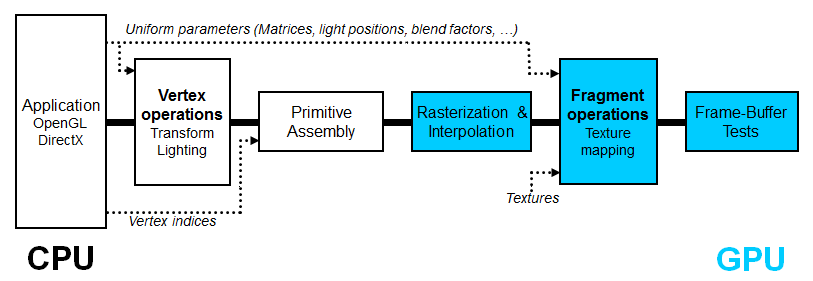
\includegraphics[width=14cm,height=50mm]{leo/images/pipeline1.png} 
1999/2000 : La deuxieme génération (Transform \& lightin par le GPU)
\\
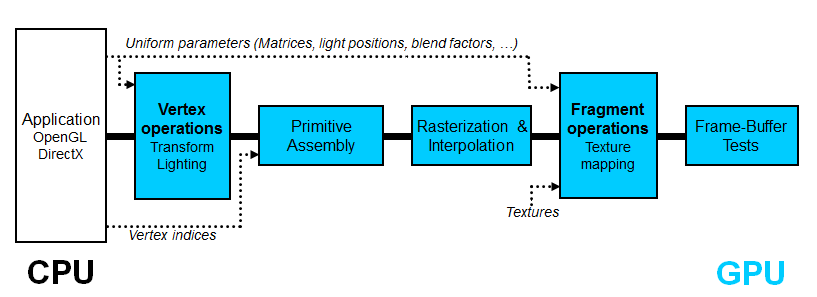
\includegraphics[width=14cm,height=50mm]{leo/images/pipeline2.png} 
2001/2002 : Troisième génération (Vertex shader par le GPU)
\\
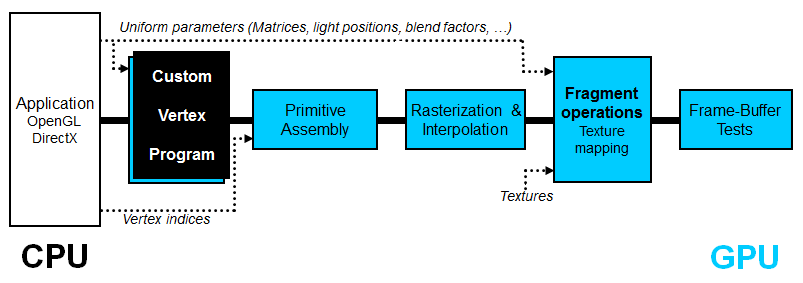
\includegraphics[width=14cm,height=50mm]{leo/images/pipeline3.png} 
2003 : Quatrième génération (Pixel shader par le GPU)
\\
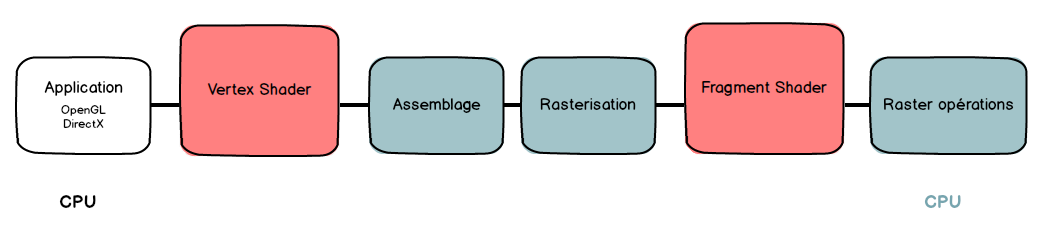
\includegraphics[width=14cm,height=50mm]{leo/images/pipeline4.png} 

\section{Deux sortes de pipeline : Fixe (FFP) et dynamique (PFP)}
Le pipeline fixe ne contient pas de shader. Il n’est donc pas programmable par les développeurs, mais est assez optimisé pour les calculs de toutes les étapes du pipeline.
\\
Au contraire, le pipeline dynamique, et ses shaders nous permettent de définir exactement le rendu à l’écran désiré. La création d’algorithmes qui diffèrent de ceux contenus dans le pipeline fixe, permet des changements au niveau de certains paramètres comme par exemple, les contrastes, les ombres, la lumière, les effets de Cell Shading ou de bump mapping…
\\
Les deux étapes programmables sont donc le vertex shader et le fragment shader ou pixel shader.
\\
Un vertex ou vertice, est un sommet d’une figure géométrique (un point particulier d’une figure).

\section{Déroulement du pipeline}
\subsection{Schéma}
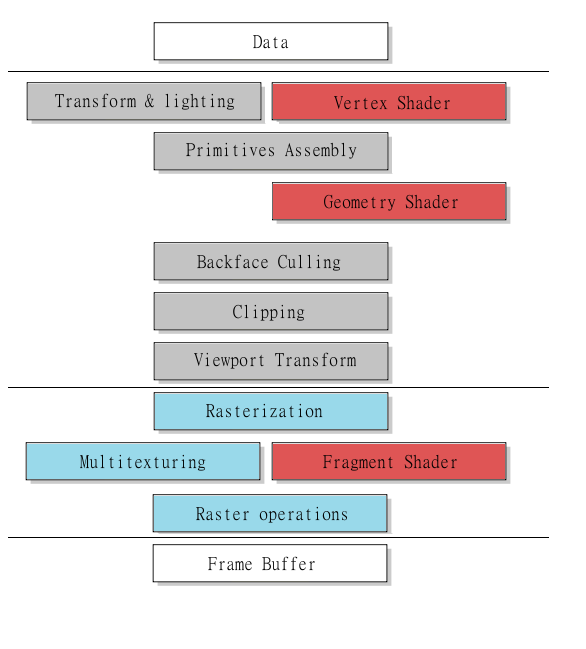
\includegraphics[width=14cm,height=180mm]{leo/images/pipeline.png}
\subsection{Définition des étapes}
\subsubsection{Data (Données brutes)}
Définition des vertices ainsi que leurs coordonnées. Ces données sont enregistrées dans un tableau de vertex (Vertex Buffer) sur le GPU. L’input assembler est le circuit qui va charger les vertices dans le pipeline à partir de l’adresse de départ du tableau. A la lecture de chaque vertice, celle-ci est passe dans le Vertex Cache. Le mémoire cache étant plus rapide, lors des utilisations ultérieures des vertices, la lecture sera plus rapide.
Chaque sommet est déclaré avec ses coordonnées x,y et z. Il peut aussi recevoir une couleur r,g,b,a, une normale Nx, Ny, Nz, une texture u,v, une taille et un poids.
\subsubsection{Transform \& lighting}
Transformation, positionnement et éclairage des sommets en passant du repère local au repère global puis dans l’espace projeté.
Cette tâche peut se décomposée en plusieurs tâches :
\\
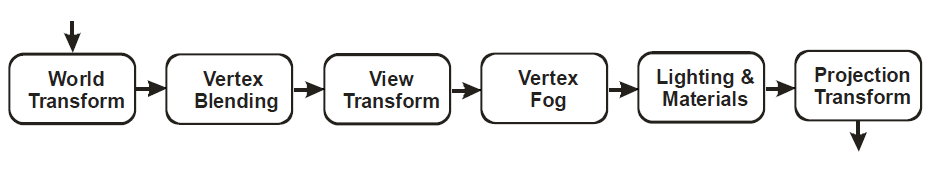
\includegraphics[width=12cm,height=35mm]{leo/images/T&L.png}
\\
\textbf{En entrée :} tableaux de coordonnées de sommets dans le repère de l’objet.
\\
\begin{itemize}
  \item{\textbf{Transform}}
Le repère local est le repère affecté à chaque objet. Chaque vertices de l’objet est localisé par rapport au centre de l’objet de coordonnées (0, 0, 0).
\\
\begin{center}
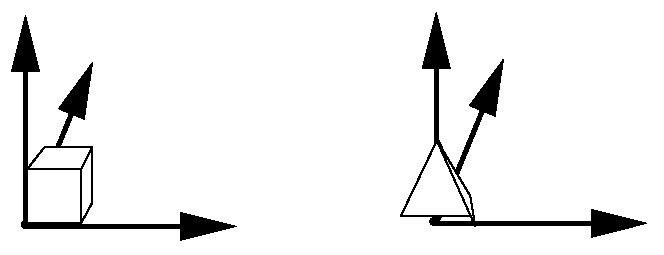
\includegraphics[width=10cm,height=40mm]{leo/images/repereLocal.png}
\end{center}

Le passage au repère global qui est le repère de la caméra, ou de l’observateur, s’exécute en changeant les coordonnées de chaque objet, qui passe donc de (0, 0, 0) à (X, Y, Z). Chaque vertice de chaque objet se met à jour en fonction des coordonnées X, Y et Z.
\\
\begin{center}
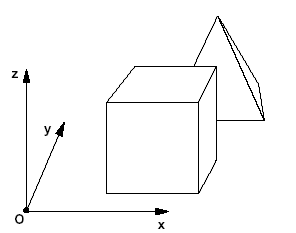
\includegraphics[width=10cm,height=60mm]{leo/images/repereGlobal.png}\\
\end{center}

Il faut que l’objet soit dans la bonne orientation, et qu’il soit au bon endroit. Cela peut nécessiter une translation, une rotation ou une mise à l’échelle. Ces opérations peuvent être effectuées sur chaque vertex, c’est-à-dire sur chaque vecteur (coordonnées X, Y et Z). Les calculs peuvent donc être parallélisés et sont effectués par le GPU. Les calculs de transformation, rotation, et de mise à l’échelle sont des multiplications de ces vecteurs par des matrices prédéfinies. Chaque opération a une matrice de multiplication prédéfinie, et des matrices existent aussi pour effectuer deux opérations en même temps.
\\
	\item{\textbf{Vertex Blending}}
Combinaison d’un ou plusieurs ensembles de sommets.
\\
	\item{\textbf{View Transform}}
Passage du repère global au repère de la caméra. Après cette transformation, le point de coordonnées (0, 0, 0) sera la caméra. La direction de la vue de l’observateur sera alignée avec l'axe de la profondeur (l'axe Z). La transformation est opérée par le même principe que le "World Transform".
\\
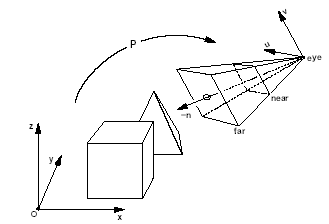
\includegraphics[width=10cm,height=60mm]{leo/images/repereCamera.png}
\\
	\item{\textbf{Vertex Fog}}
Calcul de la couleur du brouillard pour chaque sommet.
\\
	\item{\textbf{Lighting \& Materials}}
Chaque vertice fournie des couleurs RGB pour définir comment cette vertice réagie à la lumière (réflexion, teinte, contraste…). On attribut alors à la vertice une couleur RGB correspondant à son éclairage.
\\
	\item{\textbf{Projection Transform}}
Passage du repère de l'observateur à l'espace projeté.
\\
\end{itemize}
\textbf{En sortie} : sommets avec calculs d’illumination dans l’espace projeté.

\subsubsection{Primitive assembly ou Tesselation}
Assemblage des vertex sous formes de triangle. L’assemblage s’effectue en prenant les vertex dans l’ordre spécifié par le tableau de vertex.
\\\\
Il existe trois méthodes d’assemblage :
\begin{itemize}
	\item Chaque paquet de trois vertex est un triangle indépendant.
	\item Les deux derniers vertex de chaque triangle sont les deux premiers vertex d’un autre triangle (bande de triangle ou triangle strip).
	\item Le premier élément est relié à chaque paire d’élément suivant (ventilateur de triangle ou triangle fan).
	\end{itemize}
Décomposer des formes complexes, en formes géométriques simple

\subsubsection{Backface Culling}
Supprime de l’affichage les triangles qui  tournent le dos à la caméra (face arrière d’une face) en effectuant un calcul avec sa normale.
\subsubsection{Clipping}
Découpe et supprime de l’affichage les parties non visibles des objets partiellement visibles.
\subsubsection{Viewport transform}
Supprime les parties qui ne sont pas dans les coordonnées de l’écran.

\subsubsection{Rasterization}
La rastérisation, ou matricialisation, est composée du triangle setup et de l’interpolation des pixels.
\begin{itemize}
  \item{\textbf{setup ou pixellisation des triangles}} 
Utilisation de la fonction des contours : Renvoi d’un nombre entier (-1, 0, 1) pour chaque pixel en fonction d’une droite. D’un côté de la droite, -1, de l’autre, 1 et sur la droite 0.
En appliquant cette fonction aux trois segments, nous avons :
\begin{itemize}
	\item A l'intérieur du triangle, les trois fonctions (une par côté) donneront un résultat positif.
	\item A l'extérieur, une des trois fonctions donnera un résultat négatif.
\end{itemize}
Si les 3 résultats des fonctions de contours pour un pixel sont positifs, cela veut dire que le pixel appartient au triangle.
L’optimisation de ce procédé est déterminer le plus petit rectangle qui contient le triangle testé, pour exécuter le test des contours seulement sur un nombre de pixels réduit, et non sur tous les pixels de la forme.
Les tests des pixels sont exécutés parallèlement pour un gain de temps.
\item{\textbf{Interpolation}}
Chaque vertex a reçu divers paramètre comme la couleur, la profondeur. Chaque fragment  de chaque triangle, va recevoir en attributs sa couleur, sa profondeur, sa position à l’écran, une valeur de stencil, une transparence, par interpolations des trois vertices définis précédemment.
\end{itemize}
\subsubsection{Multitexturing}
Mélange des textures avec un rendu d’illumination.

\subsubsection{Raster Operations (ROP)}
Cette tâche peut se décomposée en plusieurs tâches :
\\
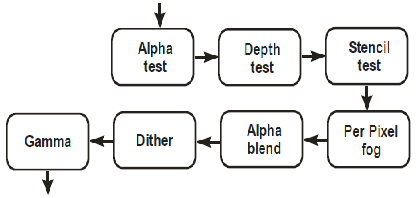
\includegraphics[width=12cm,height=40mm]{leo/images/rasterOp.png}
\\
\textbf{En entrée} : Tableau de fragment

\begin{itemize}
	\item{\textbf{Alpha Test}}
C’est le test de transparence. Certaines textures ou couleurs pouvant être transparentes, il faut pouvoir lire le canal alpha d’un pixel. Cette étape supprime tous les pixels qui n’ont pas un alpha acceptable.
\\
	\item{\textbf{Depth Test}}
C’est le test de visibilité (profondeur). C’est la coordonnée z de chaque fragment qui est comparée avec la coordonnée z des autres fragments qui sont sur le même pixel. La carte graphique utilise un depth-buffer qui est un tableau stocké en mémoire. Ce tableau va stocker pour chaque pixel la coordonnée z de l’objet le plus proche de l’écran.
C’est le circuit de gestion de la profondeur qui s’occupe de mettre à jour le depth-buffer. Il va récupérer les coordonnées du fragment reçu à l’écran, puis lire en mémoire la coordonnée z correspondante dans le tableau. Il va comparer celle-ci avec la coordonnée z du fragment reçu, et décider ou non de mettre à jour le depth-buffer et le frame-buffer.
Il faut que ces coordonnées z soient codées sur assez de bits pour avoir une bonne précision, et ne pas se retrouver avec des artefacts visuels.
\\
	\item{\textbf{Stencil Test}}
Un stencil est en  français un pochoir. C’est une sorte de masque que l’on affiche sur l’écran pour définir une vue restreinte comme une vue à travers un hublot, ou une serrure.
\\
	\item{\textbf{Per-pixel Fog}}
Cette étape permet de rajouter du brouillard (≠phénomène météorologique) sur chaque pixel. Le brouillard est ajouté grâce à une couleur de brouillard, qui est mélangée avec la couleur du pixel (moyenne). Le brouillard dépend de la profondeur du pixel. Si l’objet est proche, aucun brouillard n’est appliqué, si l’objet est trop loin, c’est seulement la couleur du brouillard qui est affiché.
\\
	\item{\textbf{Alpha Blend}}
Cette tâche sert à calculer la couleur finale du pixel. Notre GPU contient un color buffer, un tableau qui sert à stocker pour chaque pixel sa couleur finale.
Le calcul est simple, à chaque fragment envoyé :
\begin{itemize}
	\item Lecture de l’ancienne couleur du pixel,
	\item Calcul de la couleur finale en fonction du fragment envoyé et de l’ancienne couleur,
	\item Enregistrement du résultat.
\end{itemize}
Les opérations "alpha test" et "alpha blend" sont effectuées par un circuit spécialisé : le Color ROP. Il travaille en parallèle des autres tâches.
\\
	\item{\textbf{Dither}}
Mélange des couleurs des pixels adjacents pour obtenir une couleur plus consistante.
\\
	\item{\textbf{Gamma}}
Applique la correction gamma définie.
\end{itemize}
\textbf{En sortie} : le pixel prêt à être affiché relativement à l'état courant de traitement du flux de sommets.

\subsubsection{Framebuffer}
Affichage du résultat à l’écran utilisant le double-buffering, color buffer, Z-buffer.

\subsection{Fonctionnement simple}
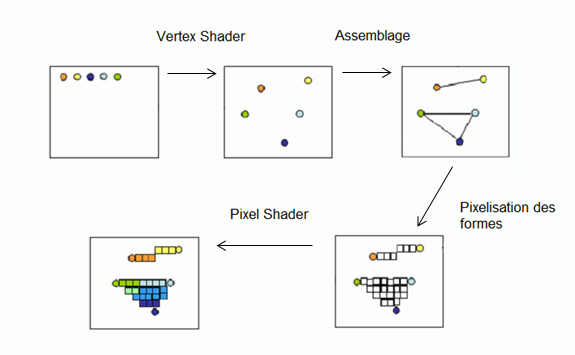
\includegraphics[width=12cm,height=60mm]{leo/images/pipelineSimple.png}


\part{Shader}
\input{leo/shader}

\part{Outils de rendu 3D}

\chapter{OpenGL}

\section{Introduction}
Comme vu précédemment l'affichage d'un contenu à l'écran par ordinateur consiste en un processus de communication entre le processeur , la carte graphique et l'écran. Ces messages, très bas niveau, sont difficilement utilisables directement par les développeurs.

OpenGL est une Interface de Programmation (API) qui définit un moyen de communication entre l'application et la carte graphique.
Cependant il n'existe aucune implémentation "officielle" d'OpenGL, c'est le rôle de chaque constructeur de l'implémenter sur son matériel.  
Elle contient un ensemble de 150 fonctions qui permettent de définir les objets et opérations nécessaires pour rendre un contexte tri-dimensionnel.
L’avantage d'OpenGL est qu’elle est totalement portable avec tous les systèmes d'exploitation. Ceci est dû au fait qu'elle sert plutôt d'intermédiaire entre l'application et le système d'exploitation. OpenGL sert à dessiner le rendu et le communiquer à la carte graphique mais ne gère ni le fenêtrage, ni les évènements. 
La majorité des bibliothèques graphiques utilisées pour créer des fenêtres graphiques gèrent OpenGL, il est donc possible d'utiliser OpenGL dans un contexte SDL, SFML, QT, API Windows.

%Device context ? Rendering context ?

OpenGL est basée sur un principe de primitives : chaque objet est composé de primitives (sommets, faces, polygones) Pour créer un objet, il suffit donc de définir toutes ses primitives.

\newcolumntype{M}[1]{>{\raggedright}m{#1}}

\begin{center}
   \begin{tabular}{| c | M{8cm} |}
   	 \hline
     \verb|GL_POINTS| 			& Dessine un point à chaque n vertex  \tabularnewline
     \hline
     \verb|GL_LINE| 			& Dessine une ligne d’un point n à n+1 \tabularnewline
     \hline
     \verb|GL_LINE_STRIP| 		& Dessine un ensemble de lignes connectées d’un vertex à un autre \tabularnewline
     \hline
     \verb|GL_LINE_LOOP| 		& Même chose que \verb|GL_LINE_STRIP|, mais du dernier vertex, on revient au premier. \tabularnewline
     \hline
     \verb|GL_TRIANGLES| 		& Dessine des triangles avec 3 vertex \tabularnewline
     \hline
     \verb|GL_TRIANGLE_STRIP| 	& Dessine une série de triangles avec les n vertexs définis   \tabularnewline
     \verb|GL_TRIANGLE_FAN| 	& Même chose que \verb|GL_TRIANGLE_STRIP|, sauf que le sommet de chaque triangle est le premier vertex défini \tabularnewline
     \hline
     \verb|GL_QUADS| 			& Dessine un quadrilatère avec 4 vertex \tabularnewline
     \hline
     \verb|GL_QUAD_STRIP| 		& Dessine une série de quadrilatères avec les n vertex définis \tabularnewline
     \hline
     \verb|GL_POLYGON| 			& Dessine un polygône générique dont le nombre de segments \verb|n’est| pas prédéterminé \tabularnewline
     \hline
   \end{tabular}
 \end{center}
 
 \begin{center}
	 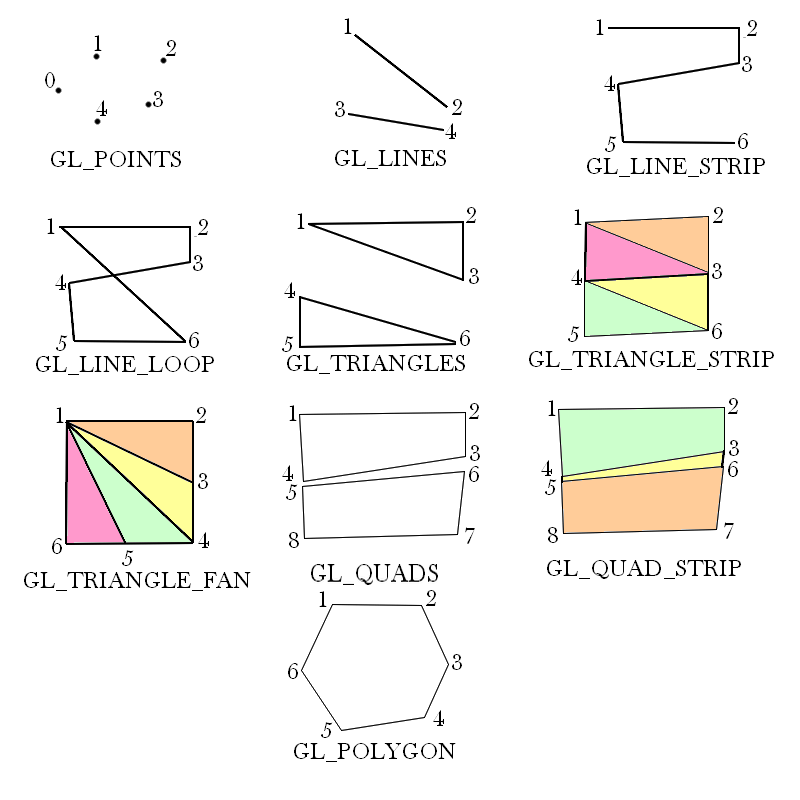
\includegraphics[height=11cm]{img/Primitives}
 \end{center}
\newpage
%Include section Intro


\section{Fonctionnement statique}
\begin{center}
	 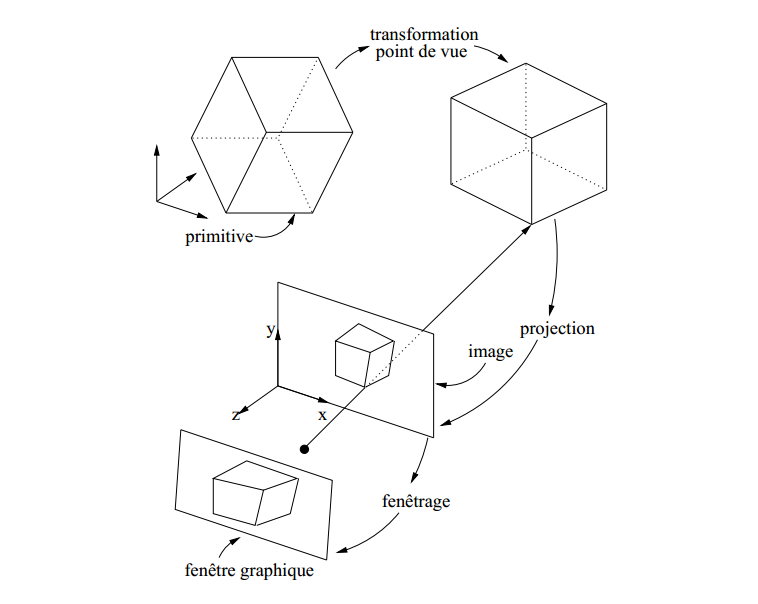
\includegraphics[height=11cm]{img/Fonctionnement}
 \end{center}

La première étape est de définir les primitives des objets à dessiner (x,y,z pour chaque Vertex).
OpenGL dessine une image tampon qui sera soit conservée dans la mémoire vidéo de la fenêtre graphique avant d’être affichée, soit une image tampon intermédiaire, on parle alors de double buffering.

La transformation du point de vue sert à la position du plan image. Elle prend en compte la position de la caméra pour se placer correctement autour de l'objet. Ces modifications sont faites à l'aide de matrices. 

Les primitives sont ensuite projetées sur ce plan en fonction des paramètres que l’on a affecté à la projection. Cette projection peut être spécifiée de deux manières. (Voir Projection)

Au final l’image que l’on obtient est redimensionnée en fonction de la taille de la fenêtre graphique . On parle maintenant de pixels et plus de vertex.
\newpage

\subsection{Primitives}
Tout d'abord, il s'agit de définir chaque objet à modéliser, grâce aux primitives précédemment décrites.

Dans le code, chaque primitives est décrite de la manière suivante:


%//////////////////////////////////
%NE PAS TOUCHER A CE TRUC IMMONDE :)
\begin{tabbing}
XXXX\=XXXX\= \kill

\> \verb|glBegin("type_de_primitive");| \\
\> \> glVertex(x,y,x);\\
\> \> . \\
\> \> . On définit chaque vertex en fonction du type de primitive\\
\> \> . \\
\> \> glVertex(x,y,x);\\
\> glEnd();
\end{tabbing}
%NE PAS TOUCHER A CE TRUC IMMONDE :)
%//////////////////////////////////

\subsection{Transformation de point de vue}
La transformation de point de vue consiste en la modification d'une matrice appelée MODELVIEW. Il faut d'abord signaler à OpenGL que l'on veut modifier cette matrice avec la fonction suivante :

\begin{tabbing}
XXXX\= \kill
\> \verb|glMatrixMode( GL_MODELVIEW );|
\end{tabbing}

Ensuite, on charge la matrice identité, ce qui permet de réinitialiser la matrice en cours, puis définit la caméra.

\begin{tabbing}
XXXX\= \kill
\> \verb|glLoadIdentity( );| \\
\> \verb|gluLookAt(eyeX,eyeY,eyeZ,centerX,centerY,centerZ,upX,upY,upZ);|
\end{tabbing}

La définition de la caméra nécessite 9 paramètres: les 3 premiers pour placer la caméra dans l'espace (x,y,z), les 3 suivants pour définir le point regardé par la caméra (x,y,z) et les trois derniers pour définir quel est l'axe vertical, en général y (On place seulement l'axe voulu à 1 et les autres à 0).\\\\

Il est possible d'effectuer d'autres opérations sur cette matrice, comme une rotation autour d'un des 3 axes ou une translation de vecteurs grâce aux deux fonctions suivantes :

\begin{tabbing}
XXXX\= \kill
\> \verb|glRotatef(angle,x,y,z);| \\\\
Avec l'angle souhaité et x, y et z à 0 ou 1 suivant autour de quel axe on souhaite\\ effectuer la rotation.\\\\
\> \verb|glTranslatef(vX,vY,vZ);|\\\\
Avec vX, vY et vZ les composantes de la translation. 
\end{tabbing}

\subsection{Projection}

La visualisation d'une scène est réalisée par deux types de transformation :

\begin{itemize}
	\item la première qui se situe dans l'espace 3D et qui permet de positionner le point de vue et si nécessaire les éclairages, pour un rendu plus réaliste (la matrice de modélisation $GL\_MODELVIEW$) que nous avons vu précédemment.

	\item la seconde qui consiste à projeter la scène 3D précédemment construite sur un plan en 2D. Sous OpenGL on retrouve deux formes de projection, la projection perspective et la projection orthographique.
\end{itemize}

La projection appliquée suite aux coordonnées des primitives est définie dans OpenGL grâce à une matrice 4x4. L'usage de ces coordonnées permet de représenter les deux types de projections sous la forme de matrices. 

\subsubsection{Perspective}
\begin{center}
	 \includegraphics[height=5cm]{img/Perspective}
 \end{center}
Notre œil perçoit ce qui loin plus petit qu’il ne l’est en réalité. Cette méthode de projection est souvent utilisée en animation, simulation et autre applications où il faudrait un degré de réalisme, comme peut le percevoir notre œil. Pour la définir il faut connaître son centre de projection (frustum), la distance entre ce point et l'objet, et enfin sa direction, qui suivra obligatoirement l’axe z. Sous OpenGL la fonction est : 
\begin{tabbing}
XXXX\= \kill
\> \verb|glFrustum(gauche, droite, bas, haut, proche, éloigné);| \\où les paramètres sont des doubles.
\end{tabbing}


\subsubsection{Orthographique}
\begin{center}
	 \includegraphics[height=7cm]{img/Ortho}
 \end{center}
Dans ce cas précis, l’image doit refléter les mesures de l’objet plutôt que son aspect réel. Contrairement à la projection en perspective la taille du viewing volume ne change pas, la distance depuis la caméra n’affecte pas la mesure de l’objet. Sous OpenGL la fonction est : 
\begin{tabbing}
XXXX\= \kill
\> \verb|glOrtho(gauche, droite, bas, haut, proche, éloigné);| \\où les paramètres sont des doubles.
\end{tabbing}

\subsection{Image Finale}

%A compléter

\newpage%Include section Fonctionnement Statique

\section{Fonctionnement dynamique}
%SHADERS

\subsection{Principe du Shader}

Le fonctionnement dynamique du pipeline graphique se différencie du fonctionnement statique par l'utilisation de shaders.
Comme expliqué précédemment les shaders sont de petits programmes écrits dans un langage spécifique : avec OpenGL, le langage utilisé est le GLSL.\\
Ils sont compilés à l'éxécution du programme OpenGL, et executés pour chaque vertex (Vertex Shader) et chaque pixel (Pixel Shader).
Ils remplacent les calculs de matrices gérés par défaut dans le fonctionnement statique d'OpenGL. C'est-à-dire qu'il faut implémenter ces calculs dans les shaders. L'intérêt est qu'il est possible d'adapter ces calculs pour satisfaire certains besoins de l'application. D'autant plus que les shaders sont exécutés par la carte graphique(GPU), qui est capable de répartir les opérations sur toutes les unités de calculs.

\subsection{Utilisation des shaders}

Il est plus ou moins aisé d'implémenter les shaders dans un programme OpenGL, suivant la bibliothèque graphique utilisée.
Nous prenons l'exemple de la SFML:\\

\begin{tabbing}
XXXX\=XXXX\= \kill\\
\> //On déclare un objet de type Shader\\
\> \verb|sf::Shader shader;|\\
\\
\>//Puis on charge les fichiers shaders\\
\> \verb|if (!shader.loadFromFile("vertex_shader.vert", "fragment_shader.frag"))|\\
\> \verb|{|\\
\> \>\verb|//error...|\\
\> \verb|}|\\
\end{tabbing}

Pour utiliser le shader il faut l'activer avant de dessiner et le désactiver quand on en a plus besoin.


\begin{tabbing}
XXXX\=XXXX\= \kill\\
\> // On active le shader\\
\> \verb|sf::Shader::bind(&shader);|\\
\\
\> ....\\
\> //On dessine nos entités OpenGL ....\\
\> ....\\
\\
\> // On désactive le shader\\
\> \verb|sf::Shader::bind(NULL);|\\
\end{tabbing}

\subsection{Exemple de Shader}
\subsubsection{Vertex Shader}

\begin{tabbing}
XXXX\=XXXX\= \kill\\
\> \verb|uniform float a;|\\
\> \\
\> \verb|void main(){|\\
\> \\
\>\> \verb|vec4 vertex = gl_Vertex;| \\
\> \\
\>\> \verb|vertex.y = vertex.y + a*cos(vertex.y)| \\
\> \\
\>\> \verb|gl_Position = gl_ModelViewProjectionMatrix * vertex;|\\
\> \\
\>\> \verb|// transforme les coordonnées de texture|\\
\>\> \verb|gl_TexCoord[0] = gl_TextureMatrix[0] * gl_MultiTexCoord0;|\\
\> \\
\>\> \verb|// transmet la couleur|\\
\>\> \verb|gl_FrontColor = gl_Color;|\\
\> \verb|}|\\
\end{tabbing}


\subsubsection{Pixel Shader}

\begin{tabbing}
XXXX\=XXXX\= \kill\\
\> \verb|uniform float a;| \\
\> \\
\> \verb|void main(){|\\
\> \\
\> \verb|gl_Position = gl_ModelViewProjectionMatrix * gl_Vertex;|\\
\> \\
\> \verb|}|\\
\end{tabbing}%Include section Fonctionnement Dynamique

%Include du fichier openGl.tex

\chapter{MatLab}
% MATLABOUNET
\section{Introduction}
MatLab ou Matrix Laboratory est un logiciel développé par la société The MathWorks, sa fonctionnalité principale est d'effectuer des calculs numériques.\\ 
Il a initialement été conçu pour faciliter le traitement des matrices, cependant il est maintenant utilisé dans tous les domaines des sciences qui nécessite de faire des calculs (par exemple le traitement d'images).\\
Dans sa dernière version MatLab peut utiliser des fonctions d'accélération par le GPU.\\


\section{Les avantages et inconvénients}
\subsection{Avantages}
\begin{itemize}
\item Temps de programmation très rapide pour les calculs et l'affichage
\item Possibilité d'inclure un programme C ou C++
\item C'est un langage interprété, donc pas de compilation
\item Une librairie et une aide très bien faite et très riche
\item Code et fonctions facillement lisibles et compréhensibles
\end{itemize}

\subsection{Inconvénients}
\begin{itemize}
\item Vitesse de calcul beaucoup moins rapide qu'en C ou C++
\item Il est payant
% A vérifier 
\item Application auto-exécutable peu pratique
\end{itemize}

\section{Conclusion}
MatLab est donc généralement utilisé pour faire des expériences en peu de temps. Certaines applications qui nécessiteraient une journée de programmation en C ou C++ peuvent se réaliser en une heure sous MatLab. En revanche, une fois programmée, le temps de calcul sous MatLab peut être cent fois supérieur à celui de C ou C++. De ce fait, MatLab ne s'utilise que très peu pour réaliser un produit finit destiné à un particulier. 

\section{Sources}
http://www.nvidia.fr/object/tesla-matlab-accelerations-fr.html
%Include du fichier matlab.tex


\part{...}
\chapter{Optimisation}
\section{Les VBO et VAO}

% ♥♥♥♥	♥♥♥♥
Les VBOs (Vertex Buffer Object) en OpenGL est une méthode qui permet d'envoyer des données vers la carte graphique, elle remplace les VA (Vertex Array) déclarés comme obsolètes par OpenGL qui étaient enregistrés sur le CPU et devaient transiter entre CPU et GPU.\\
Les VBOs ont été conçus afin d'optenir les meilleurs performances possibles. Son utilisation est actuellement la méthode la plus efficace en OpenGL car les données 3D ne résident plus dans la mémoire système mais dans la mémoire de la carte graphique ce qui permet un rendu plus rapide.
\\\\
Source : \cite{VBO}
\\\\
Les VAOs (Vertex Array Object) servent à optimiser l'utilisation des VBOs, ils sont une fonctionnalité toute nouvelle qui ressemble fortement aux Display Lists. Les VAOs permettent la "sauvegarde" de plusieurs commandes dans un seul et même objet qui lui même sera stocké dans la mémoire de la carte graphique. \\
Par exemple : ces commandes ou appels de fonctions peuvent utiliser des VBOs. Ainsi tout sera stocké directement dans la carte graphique et celle-ci n'aura plus à demander à l'application ce qu'elle doit faire. OpenGL pourra ainsi optimiser ses actions du faite qu'il connetra ses actions futurs. Ceci permet d'éviter de faire transiter trop d'informations entre le système et la carte graphique.\\\\
La création d’un VBO suit les étapes suivantes : 
\begin{itemize}
\item La génération du nouveau buffer object avec \verb|glGenBuffersARB ( );|
\item L’activation du buffer object avec \verb|glBindBufferARB ( );|
\item La copie de la donnée du vertex au buffer object avec \verb|glBufferDataARB ( );| 
\item L’usage du buffer pour le rendu de la donnée
\item La destruction du buffer
\end{itemize}
\subsubsection*{La fonction glGenBuffers} 
Créé le buffer object et retourne un nombre d’identifiants du buffer object. Deux paramètres sont attendus : 
\verb|void glGenBuffers(GLsizei n, GLuint *buffers);|
\\
Le premier, \verb|GLsizei n| où n renvoie au nombre de buffer object que l’on veut générer, et le second \verb|GLuint *buffers| qui renvoie les nombres identifiants de buffers dans un bloc mémoire commençant par buffers (élément simple ou tableau)

\subsubsection*{La fonction glBindBufferARB}

Une fois que le nom du buffer object est généré, il faut l’activer pour ensuite l’utiliser. La fonction utile est 
\begin{center}
\verb|void glBindBuffer(GLenum type, Gluint buffer) ;|
\end{center}
qui prend en compte deux paramètres. \verb|GLenum type| où type peut être \verb|GL_ARRAY_BUFFER| ou \verb|GL_ELEMENT_ARRAY_BUFFER| (d’autres types sont connus, comme \verb|GL_PIXEL_PACK_BUFFER| mais leur utilisation se fait avec le Pixel Buffer Object (PBO) que nous n’aborderons pas ici). \verb|GL_ARRAY_BUFFER| est utilisé quand le buffer object se réfère aux données des vertex (positions, couleurs, normales etc.) \verb|GL_ELEMENT_ARRAY_BUFFER| est utilisé quand les indices des vertex seront stockés dans le buffer

\subsubsection*{La fonction glBufferData}

A présent le buffer object est généré et prêt à recevoir des données. Sa taille est par défaut mise à zéro, la fonction \verb|glBufferDate| sert donc à l’initialiser avec les informations qui sont connues dans le tableau de données que l’on envoie.
\begin{center}
\verb|void glBufferData(GLenum type, GLsizeiptr size, const GLvoid * data, |\\
\verb|GLenum usage);|
\end{center}
\verb|GLenum| type est le même que celui du \verb|glBindBuffer()|, il peut prendre le paramètre \verb|GL_ARRAY_BUFFER| ou \verb|GL_ELEMENT_ARRAY_BUFFER|. \verb|GLsizeiptr size-| est la taille en bytes du tableau de vertex, \verb|const GlVoid *data| est le pointeur vers le tableau de données qui doit être copié. (Le tableau de position des vertex). Enfin usage fait référence à l’OpenGL et permet de définir l’utilisation du buffer (Voir Cas d’utilisation du buffer).
\subsubsection{Cas d'utilisation du buffer}

Le dernier paramètre de la fonction \verb|glBufferData()|, usage, est donc une indication sur la façon dont le buffer object va être utilisé . Usage fait référence à deux critères qui seront la fréquence à laquelle les informations seront modifiées et le type d’accès à ces données. Chaque constante sera la combinaison de ces deux critères et sera de la forme : \verb|GL_VALEURFREQUENCE_VALEURACCES| (cf. tableau 1 et tableau 2)
\\
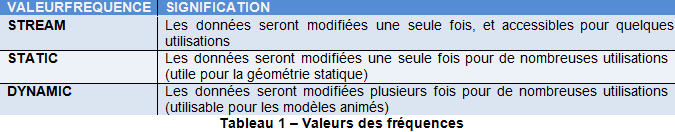
\includegraphics[width=15cm,height=2.94cm]{img/tableau1.png}
\\
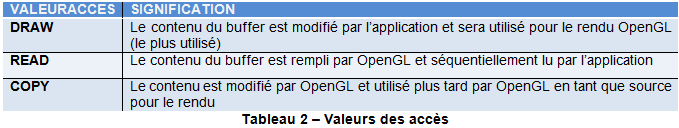
\includegraphics[width=15cm,height=3cm]{img/tableau2.png}

\subsubsection{Application d'un VA}
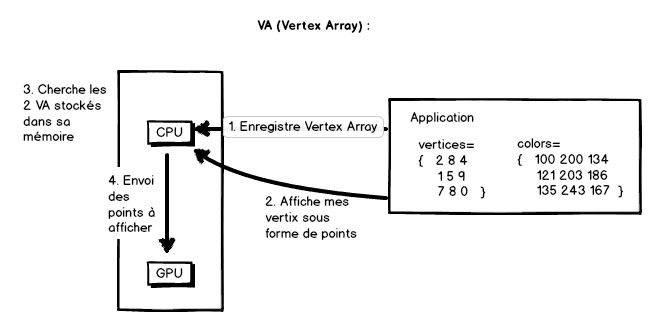
\includegraphics[width=15cm,height=7.48cm]{img/VA.png}
\subsubsection{Application d'un VBO}
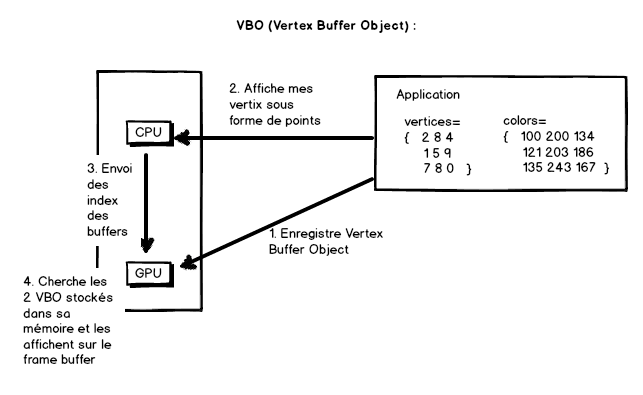
\includegraphics[width=15cm,height=9.26cm]{img/VBO.png}
\subsubsection{Application d'un VBO dans un VAO}
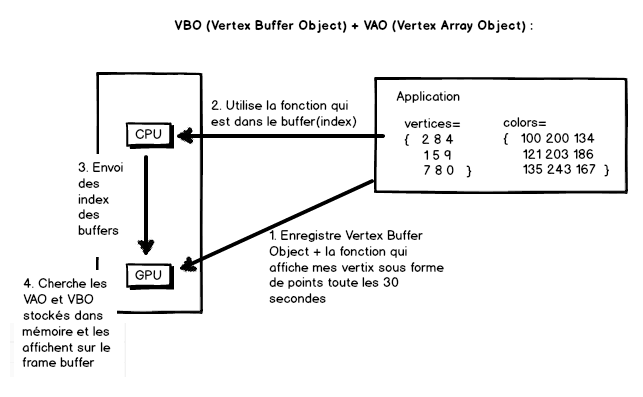
\includegraphics[width=15cm,height=9.21cm]{img/VAO_VBO.png}
%♥♥♥♥	♥♥♥♥

\part{Annexes}

\section{Exemple Structure code OpenGL}

\begin{tabbing}
XXXX\=XXXX\=XXXX\= \kill

\verb|int main(){|\\
\> \verb|//Création de la fenetre suivant la bibliotèque choisie|\\
\> \verb|//Le contexte OpenGL est défini à ce moment la par la bibliotèque|\\
\\	
\> \verb|glMatrixMode( GL_PROJECTION );//On active la matrice de Projection|\\
\> \verb|glLoadIdentity( );// On reinitialise la matrice actuelle (GL_PROJECTION)|\\
\> \verb|gluPerspective(80,(double)800/600,1,10);|\\
\> \verb|/*Définition de l'angle de vision de la caméra , du ratio de la fenetre, |\\
\> \verb|ainsi que de l'intervalle de profondeur dans lequel faire le rendu |\\
\> \verb|ici de 1 à 10.*/|\\
\\
\> \verb|glEnable(GL_DEPTH_TEST); //Activation du Z-Buffer|\\
\\
\> \verb|bool running = true;|\\
\\

\> \verb|while(running){|\\

\>\> \verb|glClear(GL_COLOR_BUFFER_BIT \GL_DEPTH_BUFFER_BIT);|\\
\>\> \verb|//Efface les buffers de couleurs ainsi que de Z-Buffer|\\
\\
\>\> \verb|glMatrixMode( GL_MODELVIEW );|\\
\>\> \verb|//On active la matrice ModelView|\\
\\
\>\> \verb|glLoadIdentity();// Réinitialise la matrice actuelle (GL_MODELVIEW)|\\
\\
\>\> \verb|gluLookAt(3,3,3,0,0,0,0,1,0);|\\
\>\> \verb|//On place la caméra en 3,3,3 dans le repère elle regarde|\\
\>\> \verb|l'origine du repère et la verticale est Y.|\\
\\
\>\> \verb|glBegin(GL_LINES);//On indique que l'on définit des lignes|\\
\>\>\> \verb|glColor3ub(0,0,255);//On change la couleur courante|\\
\>\>\> \verb|glVertex3i(0,0,0);//Ligne de ce point ....|\\
\>\>\> \verb|glVertex3i(1,0,0);//.... à ce point|\\
\>\>\> \verb|glColor3ub(0,255,0);//...|\\
\>\>\> \verb|glVertex3i(0,0,0);//...|\\
\>\>\> \verb|glVertex3i(0,1,0);//...|\\
\>\>\> \verb|glColor3ub(255,0,0);//...|\\
\>\>\> \verb|glVertex3i(0,0,0);//...|\\
\>\>\> \verb|glVertex3i(0,0,1);//...|\\
\>\> \verb|glEnd();// Fin de la définition des primitives|\\
\\
\>\> \verb|//Affichage à l'ecran en fonction de la bibliotèque|\\

\> \verb|}|\\
\> \verb|return 0;|\\
\verb|}|
\end{tabbing}
 
\newpage
\end{document}